\documentclass[brazilian, 12pt, a4paper, final]{article}
\usepackage[utf8]{inputenc}
\usepackage[brazil]{babel}
\usepackage[T1]{fontenc}
\usepackage{multicol}
\usepackage{graphicx}
\usepackage{indentfirst}
\usepackage{amsmath}
\usepackage{array}
\usepackage{caption}
\usepackage{float}
\usepackage{enumitem}
\usepackage[left=1.5cm, right=1.5cm]{geometry}

\title{\textbf{Estudo das Propriedades Analíticas e Numéricas do Mapa de Marotto}}

\author{Cristiane de Paula Oliveira\\\\\small{Instituto de Física -- Universidade Federal do Rio Grande do Sul}}

\begin{document}

\maketitle

\begin{abstract}
  \noindent
  Nestre trabalho serão estudados as propriedades analíticas e numéricas do mapa de Marotto, como pontos fixos, estabilidade dos pontos fixos  dobramento de período. Esse mapa é bidimensional e depende de dois parâmetros reais $a$ e $b$. Diferentes combinações desses parâmetros levam a comportamentos muito interessantes do mapa. \\
  \\
  \textbf{Palavras-chave:} mapa de Marotto, comportamento caótico, mapas bidimensionais
\end{abstract}
\begin{multicols*}{2}
\section{Introdução}
Em sistemas dinâmicos, mapas se referem a uma função de um sistema dinâmico discreto que evolui. Mapas podem ter diversas aplicações em diversas áreas de estudo, como física, biologia e economia. 

Neste trabalho são estudadas as propriedades analíticas e numéricas do mapa de Marotto.

\section{Mapa de Marotto}
Neste trabalho será investigado o comportamento de mapa de Marotto, dados pelo seguinte sistema discreto
\begin{eqnarray}
  x_{n+1}&=&(ax_n+by_n)(1-ax_n-by_n), \label{eq:mapax} \\
  y_{n+1}&=&x_n. \label{eq:mapay}
\end{eqnarray}
onde, $a$ e $b$ são parâmetros reais.

Esse mapa é bidimensional e, dependendo das escolhas dos parâmetros $a$ e $b$ possui comportamentos diversos, como dobramento de período e caos.

O mapa de Marotto não possui, a princício, nenhum significado físico.

\section{Pontos fixos e estabilidade}
Os pontos fixos do mapa são os pontos em que
\begin{eqnarray}
  x^{\star} &\doteq & x_{n+1}=x_{n},\\
  y^{\star} &\doteq & y_{n+1}=y_{n}.
\end{eqnarray}

No caso deste mapa, os pontos fixo acontece em
\begin{eqnarray}
	x^{\star}&=&(ax^{\star}+by^{star})(1-ax^{\star}-by^{star}), \label{eq:xx} \\
	y^{\star}&=&x^{\star}. \label{eq:yx}
\end{eqnarray}
Pode-se substituir a equação(\ref{eq:yx}) na equação (\ref{eq:xx}) para encontrar os pontos fixos. Desta forma, os pontos fixos são dados pela equação
\begin{equation}\label{eq:fix}
	x^{\star}=(a+b)x^{\star}+(a+b)^{2}x^{\star 2}. 
\end{equation}

Resolvendo a equação (\ref{eq:fix}), encontra-se que os pontos fixos são
\begin{eqnarray}
	(x^{\star},y^{\star})&=&(0,0); \label{eq:fix1} \\
	(x^{\star},y^{\star})&=&\left(\frac{a+b-1}{(a+b)^2},\frac{a+b-1}{(a+b)^2}\right) \label{eq:fix2}.
\end{eqnarray}

Para analisar a estabilidade de cada ponto fixo, é preciso analisar a matriz Jacobiana do sistema, definida como
\begin{equation}
	J(x^{\star},y^{\star})= 
	\begin{bmatrix}
		\frac{\partial F}{\partial x}\big|_{(x^{\star},y^{\star})} & \frac{\partial F}{\partial y}\big|_{(x^{\star},y^{\star})} \\
		\frac{\partial G}{\partial x}\big|_{(x^{\star},y^{\star})} & \frac{\partial G}{\partial y}\big|_{(x^{\star},y^{\star})}           
	\end{bmatrix}
\end{equation}

Sendo $F(x,y)$ dada pela equação (\ref{eq:mapax}) e $G(x,y)$ pela equação (\ref{eq:mapay}), a matriz jacobiana fica
\begin{equation}
	J(x^{\star},y^{\star})= 
	\begin{bmatrix}
		a-2a^2x-2aby & b-2b^2y-2abx \\
	 	1 & 0            
	\end{bmatrix}.
\end{equation}

Pontos fixo são assintoticamente estáveis se os autovalores $\lambda_1$ e $\lambda_2$ estiverem no intervalo $-1 < \lambda_{1,2} < 1$. Caso $\lambda_{1,2}$ estiver fora deste intervalo é instável.

No ponto $(x,y)=(0,0)$, a matriz jacobiana fica
\begin{equation}
	J(x^{\star},y^{\star})= 
	\begin{bmatrix}
		a & b \\
	 	1 & 0            
	\end{bmatrix}.
\end{equation}
Os autovalores dessa matriz são dados por
\begin{equation}
	\mathrm{det}(J-\lambda I)= 
	\begin{bmatrix}
		a-\lambda & b \\
	 	1 & -\lambda            
	\end{bmatrix}=0.
\end{equation}
Assim, a equação característica fica
\begin{equation}
	\lambda^2-a\lambda-b=0.
\end{equation}
Portanto, os autovalores são 
\begin{equation} \label{eq:auto1}
	\lambda_{1,2}=\frac{a\pm\sqrt{a^2+4b}}{2}. 
\end{equation}
Para que o ponto $(x,y)=(0,0)$ seja estável, $-1<\lambda_{1,2}<1$.

No ponto $(x,y)=\left(\frac{a+b-1}{(a+b)^2},\frac{a+b-1}{(a+b)^2}\right)$, a matriz jacobiana é dada por
\begin{equation}
	J(x^{\star},y^{\star})= 
	\begin{bmatrix}
		\frac{a(2-(a+b))}{a+b} & \frac{b(2-(a+b))}{a+b} \\
	 	1 & 0            
	\end{bmatrix}.
\end{equation}
Os autovalores são encontrados a partir de 
\begin{equation}
	\mathrm{det}(J-\lambda I)= 
	\begin{bmatrix}
		\frac{a(2-(a+b))}{a+b}-\lambda & \frac{b(2-(a+b))}{a+b} \\
	 	1 & -\lambda
	\end{bmatrix}.
\end{equation}
A equação característica para o ponto fixo $(x,y)=\left(\frac{a+b-1}{(a+b)^2},\frac{a+b-1}{(a+b)^2}\right)$ é
\begin{equation}
	\lambda^2-A\lambda-B=0.
\end{equation}
onde \begin{equation}
A=\frac{a}{a+b}(2-(a+b))
\end{equation} e \begin{equation}
B=\frac{b}{a+b}(2-(a+b)).
\end{equation}
Assim, os autovalores da matriz jacobiana são
\begin{equation} \label{eq:auto2}
	\lambda_{1,2}=\frac{A\pm\sqrt{A^2+4B}}{2}.
\end{equation}
Para que este ponto seja estável, é necessário que $-1<\lambda_{1,2}<1$.

\section{Resultados e análises}
Os gráficos a seguir mostram o comportamento do mapa bidimensional para diferentes escolhas dos parâmetros $a$ e $b$. O ponto inicial foi fixado em $x_0=y_0=0,1$ e foram executadas $N=100 000$ iterações no mapa.

%------ Ver pontos fixos e estabilidade desses gráficos ---------
Na figura \ref{fig:067} mostra-se a órbita do mapa de Marotto para $a=0,67$ e $b=2,5$. Para esses parâmetros os pontos fixos segundo as equações (\ref{eq:fix1}) e (\ref{eq:fix2}) são 
\begin{eqnarray}
	\nonumber (x^{\star}_1,y^{\star}_1)&=&(0; 0) \;\; \mathrm{e} \\
	\nonumber (x^{\star}_2,y^{\star}_2)&=&(0,21594; 0,21594).
\end{eqnarray}

\begin{figure}[H] 
  \centering
  \includegraphics[width=0.34\textwidth,angle=-90]{mapa_a067_b250.eps}
  \caption{Mapa para $a=0,67$ e $b=2,5$.}
  \label{fig:067}
\end{figure}

Pela a análise da estabilidade a partir dos autovalores da matriz, percebe-se que o ponto fixo $(x^{\star}_1,y^{\star}_1)$ é instável, pois a matriz possui autovalores $\lambda_1=3,4149$ e $\lambda_2=-2,84497$. Já o ponto fixo $(x^{\star}_2,y^{\star}_2)$ tem autovalores $\lambda_{1,2}=-0,12364\pm0,95259 i$ complexos. A norma dos autovalores $|\lambda_{1,2}|=\sqrt{a^2+b^2}$, em que $\lambda_{1,2}=a\pm b i$, tem valor $|\lambda_{1,2}|=0,96058$, indicando que esse ponto é assintóticamente estável. Na figura \ref{fig:067} é possível verificar a convergência para o ponto fixo.
   
\begin{figure}[H] 
  \centering
  \includegraphics[width=0.34\textwidth,angle=-90]{mapa_a078_b250.eps}
  \caption{Mapa para $a=0,78$ e $b=2,5$.}
  \label{fig:078}
\end{figure}

Escolhendo $a=0,78$ e $b=2,5$, obtém-se, fazendo a mesma análise anterior, que os dois pontos fixos do mapa são
\begin{eqnarray}
	\nonumber (x^{\star}_1,y^{\star}_1)&=&(0; 0) \;\; \mathrm{e} \\
	\nonumber (x^{\star}_2,y^{\star}_2)&=&(0,21193; 0,21193).
\end{eqnarray}
Novamente, o ponto fixo $(x^{\star}_1,y^{\star}_1)$ é instável, com autovalores $\lambda_1=3,57634$ e $\lambda_2=2,79634$. O ponto fixo $(x^{\star}_2,y^{\star}_2)$ possui autovalores $\lambda_{1,2}=0,15220\pm 0,975993i$, com $|\lambda_{1,2}|=0,98773$, sendo assim estável.

Quando $a=1,2$ e $b=2,5$, os pontos fixos do mapa são
\begin{eqnarray}
	\nonumber (x^{\star}_1,y^{\star}_1)&=&(0; 0) \;\; \mathrm{e} \\
	\nonumber (x^{\star}_2,y^{\star}_2)&=&(0,19722; 0,19722).
\end{eqnarray}
O ponto fixo $(x^{\star}_1,y^{\star}_1)$ é instável pois seus autovalores são $\lambda_1=3,81870$ e $\lambda_2=-2,61870$. O ponto fixo $(x^{\star}_2,y^{\star}_2)$ também é instável, possuindo autovalores $\lambda_{1,2}=0,27568\pm1,03569i$, cuja norma é $|\lambda_{1,2}|=1,07175$.

\begin{figure}[H] 
  \centering
  \includegraphics[width=0.34\textwidth,angle=-90]{mapa_a120_b250.eps}
  \caption{Mapa para $a=1,2$ e $b=2,5$.}
  \label{fig:120}
\end{figure}

Para $a=1,35$ e $b=2,5$, os pontos fixo são 
\begin{eqnarray}
	\nonumber (x^{\star}_1,y^{\star}_1)&=&(0; 0) \;\; \mathrm{e} \\
	\nonumber (x^{\star}_2,y^{\star}_2)&=&(0,19228; 0,19228).
\end{eqnarray}
O ponto $(x^{\star}_1,y^{\star}_1)$ e $(x^{\star}_2,y^{\star}_2)$ são instáveis, com autovalores $\lambda_1=3,90852$ e $\lambda_2=-2,55852$, para $(x^{\star}_1,y^{\star}_1)$, e $\lambda_{1,2}=0,32435\pm1,04695i$, com $|\lambda_{1,2}|=1,09604
$ para $(x^{\star}_2,y^{\star}_2)$.

\begin{figure}[H] 
  \centering
  \includegraphics[width=0.34\textwidth,angle=-90]{mapa_a135_b250.eps}
  \caption{Mapa para $a=1,35$ e $b=2,5$.}
  \label{fig:135}
\end{figure}

Algo bastante interessante acontece ao mapa quando $b=2,5$. Percebe-se pelas figuras \ref{fig:120} e \ref{fig:135}, onde $a=1,2$ e $a=1,35$ respectivamente, que a órbita do mapa é um ciclo. Em $a=1,2$, o ciclo é contínuo e fechado, enquanto que para $a=1,35$ o ciclo, apesar de bastante parecido com o anterior, não é contínuo.

\begin{figure}[H] 
  \centering
  \includegraphics[width=0.34\textwidth,angle=-90]{lyapunov_a00_b25.eps}
  \caption{Superior: Expoente de Lyapunov para $b=2,5$ e $a$ variável. Inferior: Diagrama de bifurcação.}
  \label{fig:25}
\end{figure}

Na figura \ref{fig:25}, é retratado o expoente de Lyapunov  no topo e o  diagrama de bifurcação no gráfico de baixo. Mantém-se o parâmetro $b$ fixo em $b=2,5$ e varia-se o parâmetro $a$. São realizadas $N=10000$ iterações no mapa, variando-se 1000 vezes o parâmetro $a$ de $a=0$ em passos de tamanho $da=0,004$.

Pelo expoente de Lyapunov e pelo diagrama de bifurcação da figura \ref{fig:250}, percebe-se que no intervalo aproximado em que $0,83<a<1,66$ o mapa possui um comportamento caótico. Em $a\approx1,66$ há um dobramento do período e em $a\approx1,70$ há outro dobramento de período da órbita. Para $a>1,85$ o mapa se torna predominantemente caótico.

\begin{figure}[H] 
  \centering
  \includegraphics[width=0.34\textwidth,angle=-90]{mapa_a080_b300.eps}
  \caption{Mapa para $a=0,8$ e $b=3,0$.}
  \label{fig:080}
\end{figure}

Na figura \ref{fig:080} mostra-se o mapa para a escolha de parâmetros $a=0,8$ e $b=3,0$ enquanto na figura \ref{fig:110} mostra-se o mapa com as escolhas $a=1,1$ e $b=3,0$. 
Os pontos fixos do mapa da figura \ref{fig:080} são
\begin{eqnarray}
	\nonumber (x^{\star}_1,y^{\star}_1)&=&(0; 0) \;\; \mathrm{e} \\
	\nonumber (x^{\star}_2,y^{\star}_2)&=&(0,19391; 0,19391).
\end{eqnarray}

\begin{figure}[H] 
  \centering
  \includegraphics[width=0.34\textwidth,angle=-90]{mapa_a110_b300.eps}
  \caption{Mapa para $a=1,1$ e $b=3,0$.}
  \label{fig:110}
\end{figure}


Tanto o ponto fixo $(x^{\star}_1,y^{\star}_1)$ quanto o ponto fixo $(x^{\star}_2,y^{\star}_2)$ são instáveis. Os autovalores do primeiro ponto fixo são $\lambda_1=3,88712$ e $\lambda_2=-3,08712$, ambos fora do intervalo $-1<\lambda_{1,2}<1$. O segundo ponto fixo possui autovalores complexo $\lambda_{1,2}=0,18947\pm1,17692i$, com $|\lambda_{1,2}|=1,19208$, também fora do intervalo de estabilidade.

Os pontos fixos do mapa da figura \ref{fig:110} são
\begin{eqnarray}
	\nonumber (x^{\star}_1,y^{\star}_1)&=&(0; 0) \;\; \mathrm{e} \\
	\nonumber (x^{\star}_2,y^{\star}_2)&=&(0,18441; 0,18441).
\end{eqnarray}

\begin{figure}[H] 
  \centering
  \includegraphics[width=0.34\textwidth,angle=-90]{lyapunov_a05_b30.eps}
  \caption{Superior: Expoente de Lyapunov para $b=3,0$ e $a$ variável. Inferior: Diagrama de bifurcação.}
  \label{fig:30}
\end{figure}

Novamente, ambos são instáveis com autovalores  $\lambda_1=4,05749$, $\lambda_2=-2,95749$ e $\lambda_{1,2}=0,28171\pm1,20716i$, com $|\lambda_{1,2}=1,23959$ fora do intervalo de estabilidade.

Na figura \ref{fig:30} mostra-se o expoente de Lyapunov e o diagrama de bifurcação para o mapa com parâmetro $b$ fixo e $a$ variando-se. Nota-se que tanto para $a=0,8$ quanto para $a=1,1$ o mapa se encontra no regime caótico. Para o valor de $b=3,0$ o mapa possui comportamento bastante complicado, sendo em sua maior parte caótico, com expoente de Lyapunov maior que zero, existindo apenas uma pequena combinação de parâmetros em que a órbita é multiperiódica.

\begin{figure}[H] 
  \centering
  \includegraphics[width=0.34\textwidth,angle=-90]{mapa_a250_b200.eps}
  \caption{Mapa para $a=2,5$ e $b=2,0$.}
  \label{fig:250}
\end{figure}

Com a escolha de parâmetros $a=2,5$ e $b=2,0$, obtém-se o mapa retratado na figura \ref{fig:250}. Os pontos fixos desse mapa são 
\begin{eqnarray}
	\nonumber (x^{\star}_1,y^{\star}_1)&=&(0; 0) \;\; \mathrm{e} \\
	\nonumber (x^{\star}_2,y^{\star}_2)&=&(0,17284; 0,17284).
\end{eqnarray}

Ambos os pontos fixos são instáveis. Os autovalores do ponto fixo $(x^{\star}_1,y^{\star}_1)$ são	$\lambda_1=4,34233$ e $\lambda_2=-1,84233$. Os autovalores complexos do ponto fixo $(x^{\star}_2,y^{\star}_2)$ são $\lambda_{1,2}=0,69444\pm 0,79301i$, com $|\lambda_{1,2}|=1,05409$.

Na figura \ref{fig:20} mostra-se o expoente de Lyapunov e o diagrama de bifurcação do mapa para $b=2,0$. Percebe-se que há um dobramento de período em $a\approx1,85$, $a\approx2,18$ e $a\approx2,27$. Após, o mapa se torna caótico. A escolha de parâmetro $a=2,5$ está nessa região caótica.

\begin{figure}[H] 
  \centering
  \includegraphics[width=0.34\textwidth,angle=-90]{lyapunov_a00_b20.eps}
  \caption{Superior: Expoente de Lyapunov para $b=2,0$ e $a$ variável. Inferior: Diagrama de bifurcação.}
  \label{fig:20}
\end{figure}



Na figura \ref{fig:380} é mostrado o mapa para os parâmetros $a=3,8$ e $b=0,5$.
Os pontos fixos do mapa são 
\begin{eqnarray}
	\nonumber (x^{\star}_1,y^{\star}_1)&=&(0; 0) \;\; \mathrm{e} \\
	\nonumber (x^{\star}_2,y^{\star}_2)&=&(0,17847; 00,17847).
\end{eqnarray}

\begin{figure}[H] 
  \centering
  \includegraphics[width=0.34\textwidth,angle=-90]{mapa_a380_b050.eps}
  \caption{Mapa para $a=3,8$ e $b=0,5$.}
  \label{fig:380}
\end{figure}



O ponto fixo $(x^{\star}_1,y^{\star}_1)$ é instável, pois seus autovalores são $\lambda_1=4,26854$ e $\lambda_2=-0,46854$. O ponto fixo $(x^{\star}_2,y^{\star}_2)$ também é instável com autovalores reais $\lambda_1=1,89114$ e $\lambda_2=0,14142$.

O expoente de Lyapunov e o diagrama de bifurcação do mapa para $b=0,5$ são mostrados na figura \ref{fig:05}.

\begin{figure}[H] 
  \centering
  \includegraphics[width=0.34\textwidth,angle=-90]{lyapunov_a00_b05.eps}
  \caption{Superior: Expoente de Lyapunov para $b=0,5$ e $a$ variável. Inferior: Diagrama de bifurcação.}
  \label{fig:05}
\end{figure}

Existe uma bifurcação em $a\approx2,91$, outra em $a\approx3,36$ e outra em $a\approx3,45$. A partir daí o mapa se torna predominantemente caótico, região onde se encontra a escolha $a=3,8$.

\section{Considerações finais}

Neste trabalho foi estudado as propriedades analíticas e numéricas do mapa de Marotto. Observou-se que para diferentes escolhas dos parâmetros reais $a$ e $b$ o mapa apresentava comportamento bem diversos e interessantes. Para cada escolha de $a$ e $b$ encontrou-se os pontos fixos do mapa e foi estudado sua estabilidade. Para um valor de $b$ fixo, variou-se o parâmetro $a$ e foram construídos gráficos com o expoente de Lyapunov, cujo valor indica onde há dobramentos de período e comportamento caótico, e diagramas de bifurcação, que também auxiliam na identificação desses comportamentos.

Apesar de o mapa de Marotto não ter nenhum significado físico ou biológico, este mapa possui comportamentos que podem ser aplicados em outros campos de estudo.
 
\begin{thebibliography}{n}
\bibitem{Marotto}  F. R. ~Marotto. {\em Snap-Back Repellers Imply Chaos in ${\rm I\!R}^{n}$}, Journal of Mathematical Analysis and Aplications {\bf 63}, 199-223 (1978)
 
\bibitem{Paper} S. M. ~Salman, A. A. ~Elsadany. {\em On the bifurcation of Marotto’s map and its application in image encryption}, Journal of Computational and Applied Mathematics {\bf 328}, 177–196 (2018)

\bibitem{Book} L. H. A, ~Monteiro. {\em Sistemas Dinâmicos}, (editora Livraria da Física, 3ª edição, 2011)
  
\end{thebibliography}
\end{multicols*}

\appendix
\section{APÊNDICE - INSTRUÇÕES}

Para compilar e rodar todos os programas utiliza-se o script:
\begin{verbatim}
$ sh Marotto.sh
\end{verbatim}
É necessário variar-se os valores dos parâmetros $a$ e $b$ manualmente.

Ao final, plota-se os gráficos utilizando:
\begin{verbatim}
gnuplot> load 'PlotAll.gnu'
\end{verbatim}

\end{document}
